\documentclass[12pt]{article}
\usepackage[utf8]{inputenc}
\usepackage{ragged2e}
\usepackage{blindtext}
\usepackage{graphicx}
\usepackage{lipsum}
\usepackage{placeins}
\usepackage{algorithm}
\usepackage{algorithmic}
\usepackage{algpseudocode}
\usepackage{blindtext}
\usepackage{setspace}
\usepackage{listings}
\renewcommand{\baselinestretch}{2.5}
\usepackage[nopar]{lipsum}

\title{Fighting Wario}
\author{Computer Science Project}
\date{By Zoirjon Imomaliev}
\begin{document}

\maketitle
%\begin{flushleft}
\begin{center}
    Name: Zoirjon Imomaliev
    \\
    
    Centre Number:10816
    \\
    
    Candidate Number:
    \\
%\end{flushleft}
\end{center}
\newpage
\tableofcontents
\newpage

\section{Analysis}

\subsection{Problem Analysis}
Due to the rapid development and expansion in the technological sector in the past decade, we are presented with unlimited amount of opportunities. Operations that we were deemed 'impossible' few decades ago, such as 'Video Calling', are now a norm in our day and age. The development of the technological field has also made it impossible for a human being to live a day-to-day life without an online presence which requires a smart phone, laptop or some kind of technical device. This online presence can take place in many social media applications; Most popular being 'Facebook', 'Instagram' and 'Whats App'.
\\

Although there are numerous positive consequences that are results of our constant online presence and dependence on the technology, like 'working from home', there are also some negative consequences. One of the biggest negatives being the stress that social media exerts onto its users. Even though stress can be helpful, constant supply of it could be detrimental for our mental health, especially for the younger children who are now constantly on social media from a very early age.
\\

What can we do to cope with stress? One of the ways billions of people do so, is through video games. Playing video games is a great option in order to relax and release some stress after long, mundane and arduous day of work. Due to the high demand, there are thousands of games to choose from; However most favoured ones, like 'Fortnite', 'Fifa', or 'League of Legends',  are usually very hardware and software demanding. This is due to the high level of competition in the gaming sphere, as games try to become increasingly realistic. 
\\

A lot of my friends back home will love to game but they do not own a device that will allow them to comfortably play those high-graphics game. There is a large number of low-level graphics games that are very entertaining and enjoyable. Some of those games are 'Fireboy and Watergirl', 'Pacman' and 'Mario'. I was inspired by those types of games, with  simple, yet fun game-play that does not require the user to spend tens of hours on the game, just to be able to play it. Hence why, I made my game very simple, only asking the player to move the player in four basic directions, and avoid notorious enemies on their path. 
\\

The game itself is relatively simple, yet still amusing. It consists of a platform, where a player has simple options to control their character, in order to move it in the basic four directions, while avoiding getting attacked by the vicious enemies that are hunting the player or a player can also shoot those enemies in order to eliminate them. The player will get points depending on their progress into the game. During their progress, players can further collect different items that help boost different attributes for a period of time, such as health or speed. 
\\

However, the main problem with platform games is that few of those games are very overused, such as 'Mario'. In order to stay creative, I carried out an extensive research in order to find older platform games ,that were seen as 'legendary' at that time, and bring them back to our modern society and try to give people a new taste of the platform games.
\newpage

\subsection{Computational Suitability}
Many of the modern games are made by translating real life games into code and give the players ability to be able to keep playing their most loved games inside their computers. However, many other games, including my game, are originally made for virtual experience only. It is very challenging to have layers of platforms, that people can jump up and down from while eliminating their enemies and collecting items that boost their attributes and most importantly losing their lives when hit. 
\\

The execution of that concept is tailor made for a computer. It is easily playable, does not take lots of ram and does not require heavy computational power. It is really efficient, as you can compete with your friends to see who is able to achieve a higher score, and establish their superiority and most importantly the lives of players is not at risk at any point during the game. Furthermore, usage of a computer to execute this game allows developers to add more view capturing and captivating visual effects of characters, grass and many more real life objects. Finally, the game being easily run on most machines allows millions if not billions around the world to easily download and play this game, without leaving their house, which brings joy to all communities and people around the world, without additional costs embedded.

\subsection{Research}
There are millions of different platform based games available, one of the most recognisable ones being 'Mario' and 'Subway Surf'. Mario allows the player to control their character in a 2D, multi-layer environment in order to jump and avoid the enemies while collecting some sort of points. However, 'Subway Surf' is a game, where player is in a 3D, dynamic environment constantly faced with moving obstacles , like trains, coming directly at the player, forcing them to react quickly, tactically and efficiently. 
\\

There is a lot that I can learn from these games. Firstly, the games can have a basic goal for the player and still manage to provide highly entertaining experience. For example, in 'Mario' it is as simple as jump over enemies and collect coins, no extra complications or high skill maneuvers required to pass levels, hence it allows more people to start playing the game without the feeling of large lack of skill, which ultimately disengages the new users from play that game again. Secondly, I can see how a large problem such as a game, can be broken down into smaller problems, hence abstracted. This will make it easier for me to build and test individual parts of the game, which will increase the my efficiency while coding and debugging.
\\

My solution differs from these games due to the difference in the abilities of the character and the computer requirements. In my game, the user can also shoot the enemies that are on there to attempt to take the lives of the player and ultimately stop them form progressing. Furthermore, my game will be much smaller than 'Subway Surf' and 'Mario' and will require much less computational power in order to have an optimal and enjoyable experience while playing the game.

\subsection{Stakeholders}
Billions of young children including myself, did not have a fortunate upbringing where our financial situation would allow us to spend hundreds of pounds on expensive computationally powerful machines in order to play all the modern games. This led to me and my friends sticking to playing simple games that were not heavy on graphics and processing, yet still provide equal or more fun.\\

This was a major factor that pushed towards making a simple game, in order for billions of people around to world to be able to enjoy gaming experience without spending a large amount of money. Therefore, my main stakeholders are the children around my neighbourhood, who will greatly appreciate the game that will allow them to gain new experience with a slight competition amongst each other.


\section{Interviews}
\subsection{Summary of Interview 1}
My friends are passionate fans of 2D platform games which do not require a powerful computing unit. They also found games like 'Mario' most interesting, due the competitive environment against enemies or having a clear goal. This is what inspired me to design and plan my game to attempt to satisfy these requirements.


\newpage
\section{Requirements}
\begin{itemize}
    
    \item[Must Have]:
    \begin{enumerate}
        \item Have a fixed screen resolution(1200x704), maintains equal size on all devices
        \item Have a fixed FPS(60), ensures the game is run smoothly on all devices
        \item Player can exit the game
        \item Player sprite is displayed on the screen
        \item Enemy sprite is displayed  on the screen
        \item Player has the ability to move Left, Right, Up and Down
        \item Player has the ability to fire bullets
        \item Player sprite cannot go outside the fixed resolution
        \item Enemy sprite cannot go outside the fixed resolution
        \item Player sprite can collide with bullets
        \item Enemy sprite can collide with bullets
    \end{enumerate}
    \item[Should Have]:
    \begin{enumerate}
        \item Player health is displayed on the screen
        \item Enemy health is displayed on the screen
        \item Enemy sprite has a complex algorithm to dodge Player bullets
        \item Enemy sprite has a complex algorithm to fire bullets at the Player
        \item Elementary graphics, ensures the game is run smoothly
        \item Health aid is randomly spawned on each side
        \item Sound effects present when the Player shoots
        \item Sound effects present when the Enemy shoots
        \item Sound effects present when the Player gets hit
        \item Sound effects present when the Enemy gets hit
        \item Player can lose lives 
        \item Enemy can lose lives
        \item Player can gain health by collecting the health aid
        \item Enemy can gain health by collecting the health aid
    \end{enumerate}
    \item[Could Have]:
    \begin{enumerate}
        \item Have a trained model that opposes the player
        \item Different levels, with ascending difficulty
        \item Player can adjust the difficulty level
        \item In-game background, to make the gaming experience more engaging
        \item Allow the player to save the progress
        \item Have a pause option
        \item Advanced level graphics, to make the gaming experience more amusing
        \item Player can change the appearance of the spaceship
        \item Tutorial, to give a brief introduction to the game
        \item Full screen mode, to fully immerse the player into the game
        \item Have a multiplayer mode. to play against a real person
    \end{enumerate}
    \item[Won't Have]:
    \begin{enumerate}
        \item Online multiplayer mode, to play against a real opponent online
        \item 3D interface, to make the graphics look more realistic
        \item Player movement controlled via an external device, like a controller
        \item Implementation of an AI, in order to analyse player's moves, to have more accurate aim
        \item Mods, to allow the player to customise and add their own features to the game
        \item Settings option, to change the FPS of the game
    \end{enumerate}
\end{itemize}

\subsection{Hardware Requirements}
\begin{itemize}
    \item Minimum CPU : i3 or above 
    \item Minimum Clock Speed : 1GHz or more
    \item Minimum HDD : 50GB or more
    \item Minimum RAM : at least 1GB or higher
    \item Input : Keyboard 
    \item Output : Screen 
\end{itemize}
\\

\subsection{Software Requirements}
\begin{itemize}
    \item OS : Windows, Mac-OS or Linux
    \item IDE : e.g Visual Studio, PyCharm and etc.
    \item python installed
    \item python libraries : pygame, os, math, json, random
    \item access to the internet
\end{itemize}

\newpage
\section{Design}
\subsection{Interface}
Hand drawn diagram to display the appearance of the game to the player
\begin{figure}[H]
    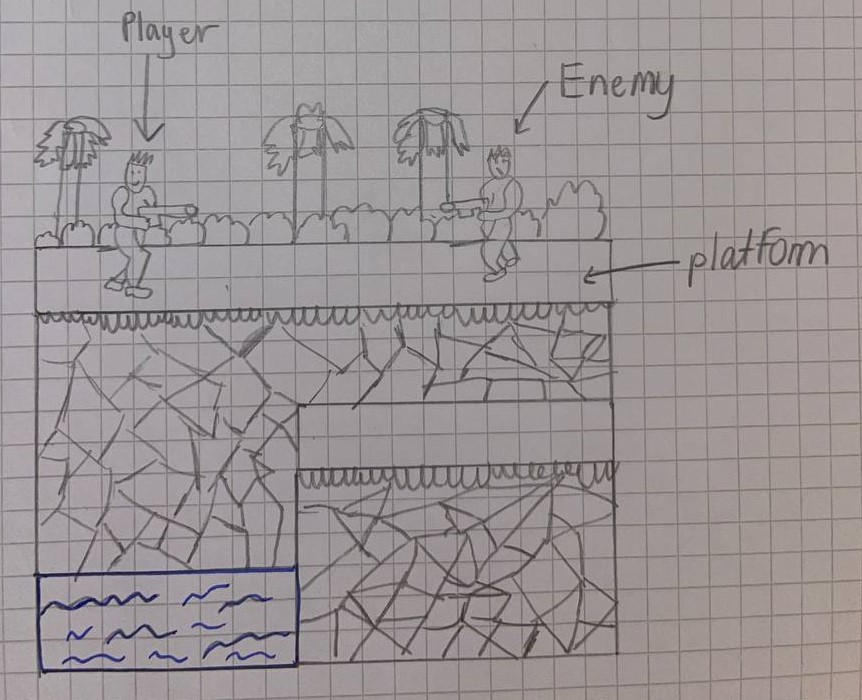
\includegraphics[width = 15cm]{designcontra.jpg}
    \centering
\end{figure}
\FloatBarrier


\newpage
\subsection{Attributes and Methods}
I used the following structure to display my Classes, Attributes and Methods
\begin{table}[H]
    \centering
    \resizebox{6cm}{!}{%
    \begin{tabular}{|c|}
    \hline
    Class & \\
    \hline
    Attributes \\
    \hline
    Methods() \\
    \hline
\end{tabular}
    \label{tab:my_label}}
\end{table}

\begin{table}[H]
    \centering
    \resizebox{6cm}{!}{%
    \large
    \begin{tabular}{|c|}
    \hline
    Game() \\  
    \hline
    width \\
    height \\
    hasGameEnded  \\
    background  \\
    FPS \\
    lives\\
    bullets\\
    \hline
    main() \\
    draw() \\
    \hline
\end{tabular}
    \label{tab:my_label}}
\end{table}

%Player Class
\newpage
This class is required to achieve following requirements:\\
Must : 3,4,6,7,8,10\\
Should : 1,7,9,11\\
This further allows me to abstract each entity into a class, using an Object Oriented Approach, in order to define all sprites from one section of code\\
\begin{table}[H]
    \centering
    \resizebox{6cm}{!}{%
    \large
    \begin{tabular}{|c|r|}
    \hline
    Player()\\
    \hline
    velocity \\
    image \\
    width  \\
    height  \\
    health \\
    posY\\
    posX\\ 
    \hline 
    init() \\
    movement() \\
    getX() \\
    getY() \\
    updateHealth() \\
    \hline
\end{tabular}
    \label{tab:my_label}}
\end{table}
\\
%Enemy class
This class is required to achieve following requirements:\\
Must : 5,9,11\\
Could : 2,3,4,8,10,12\\
I continue using an OOP approach through my program
\begin{table}[H]
    \centering
    \resizebox{6cm}{!}{%
    \large
    \begin{tabular}{|c|}
    \hline
    Enemy() \\  
    \hline
    velocity \\
    image \\
    width  \\
    height  \\
    health \\
    posX\\
    posY\\
    \hline
    init() \\
    movement() \\
    getX() \\
    getY() \\
    updateHealth() \\
    \hline
\end{tabular}
    \label{tab:my_label}}
\end{table}

%Bullet class
This class is required to achieve following requirements:\\
Must : 7,10,11\\
Could : 7,8,9,10\\
This class is very useful, as it is equally used by both Enemy and Player class
\begin{table}[H]
    \centering
    \resizebox{6cm}{!}{%
    \large
    \begin{tabular}{|c|}
    \hline
    Bullet() \\  
    \hline
    speed \\
    height \\
    bullets\\
    \hline
    getVelocity() \\
    setVelocity() \\
    checkCollision() \\
    \hline
\end{tabular}
    \label{tab:my_label}}
\end{table}

%Item class
This is required to achieve following requirements:\\
Should : 6,13,14\\
\begin{table}[H]
    \centering
    \resizebox{6cm}{!}{%
    \large
    \begin{tabular}{|c|}
    \hline
    Items() \\  
    \hline
    clock \\
    location \\
    value  \\
    \hline
    checkCollisionItems() \\
    updateHealth() \\
    spawnItem() \\
    getX()\\
    getY()\\
    \hline
\end{tabular}
    \label{tab:my_label}}
\end{table}
\newpage
I defined a tile, which will help me control the size and graphics of the game.\\
It satisfies:
\begin{table}[H]
    \centering
    \resizebox{4cm}{!}{%
    \large
    \begin{tabular}{|c|}
    \hline
    Tile() \\  
    \hline
    image \\
    rect \\
    \hline
    update() \\
    \hline
\end{tabular}
    \label{tab:my_label}}
\end{table}

\FloatBarrier
\begin{table}[H]
    \centering
    \resizebox{4cm}{!}{%
    \large
    \begin{tabular}{|c|}
    \hline
    Level() \\  
    \hline
    display surface \\
    world shift \\
    tempx \\
    dead \\
    \hline
    setup() \\
    scroll x() \\
    horizontal collision() \\
    vertical collision() \\
    player death() \\
    run() \\
    \hline
\end{tabular}
    \label{tab:my_label}}
\end{table}
\FloatBarrier

\begin{table}[H]
    \centering
    \resizebox{4cm}{!}{%
    \large
    \begin{tabular}{|c|}
    \hline
    Button() \\  
    \hline
    width\\
    height\\
    image\\
    rect\\
    clicked\\
    \hline
    draw() \\
    \hline
\end{tabular}
    \label{tab:my_label}}
\end{table}
\FloatBarrier


\subsection{Functionality}
\subsubsection{Defining the Player class}
\begin{verbatim}
    class Player(pygame.sprite.Sprite):
    def __init__(self,pos):
        super().__init__() #inherited from a sprite superclass

        #init functions
        self.import_animations()

        #player animations
        animation_indx = 0     #shows
        animation_vel = 0.15   #how quickly the images change
        image = self.animations['idle'][self.animation_indx] 
        #initial image
        

        #player structure attributes
        rect = image.get_rect(topleft = pos)  
        #blits the self.img to my player sprite

        #mechanics
        direction = pygame.math.Vector2(0,0)
        speed = 8
        jump_h = -16 # how much player jumps up
        gravity = 0.8  # the gravity on the player 

        #player directions
        movement = 'idle' #initial movement
        right = True   #initial direction player is facing
        floor = False
        ceiling = False
        rwall = False
        lwall = False

\end{verbatim}

\subsubsection{Defining the Tile class}
\begin{verbatim}
    class Tile(pygame.sprite.Sprite):
    def __init__(self, pos, size):

        #initialise pygame using super as its a parent class
        super().__init__()
        
        #new attributes for each tile that will make up my map
        image = pygame.Surface((size, size))
        image.fill('black')
        rect = self.image.get_rect(topleft = pos) 
        #pygame uses top left orientation 
        
\end{verbatim}
\subsubsection{Defining the Button class}
\begin{verbatim}
    class Button():
    def __init__(self, x, y, image, scale):
	    width = image.get_width()
		height = image.get_height()
		image = pygame.transform.scale(
            image, (int(width*scale),int(height*scale)))
		rect = image.get_rect()
		rect.topleft = (x, y)
		clicked = False
\end{verbatim}
\subsubsection{Change the x and y position of objects}
\begin{verbatim}
     item movement(keysPressed)
        IF 'a' pressed and player is in bounds THEN
            move left[West]
       
        IF 'd' pressed and player is in bounds THEN
            move right[East]
      
        IF 'w' pressed and player is in bounds THEN
            move up[North]
      
        IF 's' pressed and player is in bounds THEN
            move down[South]
\end{verbatim}
\subsubsection{Get function for position}
\begin{verbatim}
     item getX()
        return posX
    
    item getY()
        return posY
\end{verbatim}
\subsubsection{Change players health attribute}
\begin{verbatim}
     item updateHealth()
        IF Player collides with a bullet THEN
            player.health -1
        IF Enemy collides with a bullet THEN\\
            enemy.health -1
\end{verbatim}
\subsubsection{Get velocity of the player}
\begin{verbatim}
     item getVelocity()
        return velocity
\end{verbatim}
\subsubsection{Set velocity of the player}
\begin{verbatim}
    item setVelocity(x)
        set velocity to x 
\end{verbatim}
\subsubsection{Check for a collision}
\begin{verbatim}
    item checkCollisionsItems()
        IF player collides with item THEN
            player.health +1
               
\end{verbatim}
\subsubsection{Generate items}
\begin{verbatim}
    item spawnItem()
        FOR x in range 0 to width
            x = random number
            
        FOR y in range 0 to height
            y = random number
    
        assign a new location value of (x,y)
        spawn a new item at that location 
\end{verbatim}
\subsubsection{Import animations}
\begin{verbatim}
     import animations()
        folder path = 'path'
        animations = {'idle:[],'run':[],'jump':[],'fall':[]}

        for animation in animations.keys():
            f path = folder path + animation 
            animations[animation] = lol(f path)
\end{verbatim}
\subsubsection{Animate the player sprite}
\begin{verbatim}
    animate()
        current pic = animations[player movement]

        #loop over images
        animation indx += animation vel
        if animation indx >= len(current pic)
            animation indx = 0

        #update the image
        temp = current pic[int(animation indx)]
        if right then 
            image = temp
        else
            image = pygame.flip(temp,True,False)#item x,y

        #redefine the rectange
        if floor and rwall then
            rect = image.get_rect(bottomright = rect.bottomright)
        elif floor and lwall then
            rect = image.get_rect(bottomleft = rect.bottomleft)
        elif floor then
            rect = image.get_rect(midbottom = rect.midbottom)
        elif ceiling and rwall then
            rect = image.get_rect(topright = rect.topright)
        elif ceiling and lwall then
            rect = image.get_rect(topleft = rect.topleft)
        elif ceiling then
            rect = image.get_rect(midtop = rect.midtop)
\end{verbatim}
\subsubsection{Update player gravity}
\begin{verbatim}
    player gravity()
        #y-direction indicates the current vertical vector direction 
        direction.y += gravity
        rect.y += direction.y
\end{verbatim}
\subsubsection{Get players state of movement}]
\begin{verbatim}
    get movement()
        #if player is going up
        if direction.y < 0 then 
            movement = 'jump'
        elif self.direction.y > 1 then 
            movement = 'fall'
        else:
            if direction.x == 0 then
                movement = 'idle'
            else:
                movement = 'run'
\end{verbatim}
\subsubsection{Change players state when it jumps}
\begin{verbatim}
    player jump()
        #simple jump where direction is vertically up, 
        but y-value decreases as pygame 
        is reversed coordinate system
        direction.y = jump_h
\end{verbatim}
\subsubsection{Import all images from a folder}
\begin{verbatim}
    import folder(path)
    surface_list = []
    #the folder must only contain images, as any other format file 
    will cause an import error
    folder = os.walk(path)
    for a,b, imgs in folder:
        #loop through the imgs
        for img in imgs:
            full_path = path + '/' + img 
            #to handle png images with 
            transparent background
            surface = (pygame.image.load(full_path)).convert_alpha() 
            surface_list.append(surface) 

    return surface_list
\end{verbatim}
\subsubsection{Draw all spritews and objects} 
\begin{verbatim}
    #procedure to draw all sprites and objects onto the screen
    item draw() 
        display a background image using .blit() function
        draw the player onto the screen
        draw the enemy onto the screen
        draw the bullets onto the screen
        draw the health counters onto the screen
\end{verbatim}
\subsubsection{Define a map}
\begin{verbatim}
    levOne_map = [
    '                                  ',
    '                                  ',
    '                                  ',
    ' XX    XX             XX    XX    ',
    ' XX P      X      XX              ',
    ' XXXX         XX         XX       ',
    ' XXXX       XX      X      XX     ',
    ' XX    X  XXX     XX   X    XX    ',
    '       X  XXXX    XX  XXX   XXX  X',
    '   XXXX  XXXXXX  XX  XXX    XXX   ',
    ' XXXXXX   XXXXX   X  XXX    X X   ']

    
    #parameters that are used across the game
    tileDim = 64
    scr_width = 1200
    scr_height = len(levOne_map) * tileDim
\end{verbatim}
\subsubsection{Main loop for the game}
\begin{verbatim}
    item main() 
        WHILE the game is running:
            fill the background with a given colour

            Check if game is paused:
                Draw menu buttons
                Check if menu_state = 'main' then
                    close the menu screen
                Check if menu_state = 'options' then
                    open new menu screen with different options
                Else
                    run the Game and close the menu
                
            Poll for events in pygame        
                If keys are pressed THEN
                    If escape button pressed THEN
                        game_paused = 'True'
                If event is pygame.quit THEN
                    quit pygame
                    call sys exit 

            Update the display
            Set clock tick to 60
\end{verbatim}

\subsection{Test Plan}
\begin{itemize}
    \item Need to check code and compare against the requirements
    \item Carry out multiple iterations, each stage improving the game
    \item test for crucial conditions such as collisions of the player, health of the player and the enemy
\end{itemize}


\section{Implementation}
\subsection{Iteration 1}
\subsubsection{Game Class}
Whenever I tackle a problem, small or large I approach it from different perspectives. Depending on the problem or tasks complexity and functionality I carefully choose the type of programming paradigm that is most appropriate for its implementation. Here, the problem is relatively large, so like most of times, I will develop this game using object oriented techniques otherwise known as OOP. On practical basis it will allow me to break my large problem of a game into much smaller sub-problems that are easier to code, debug and test, hence help me abstract the problem.

Firstly, I needed some basic conditions to be met, to even run my program.
I imported a python library named 'pygame' ,which is what I will be using to implement my game, then I implemented a basic loop, to execute my program.
\newpage

\begin{figure}[H]
\begin{center}
    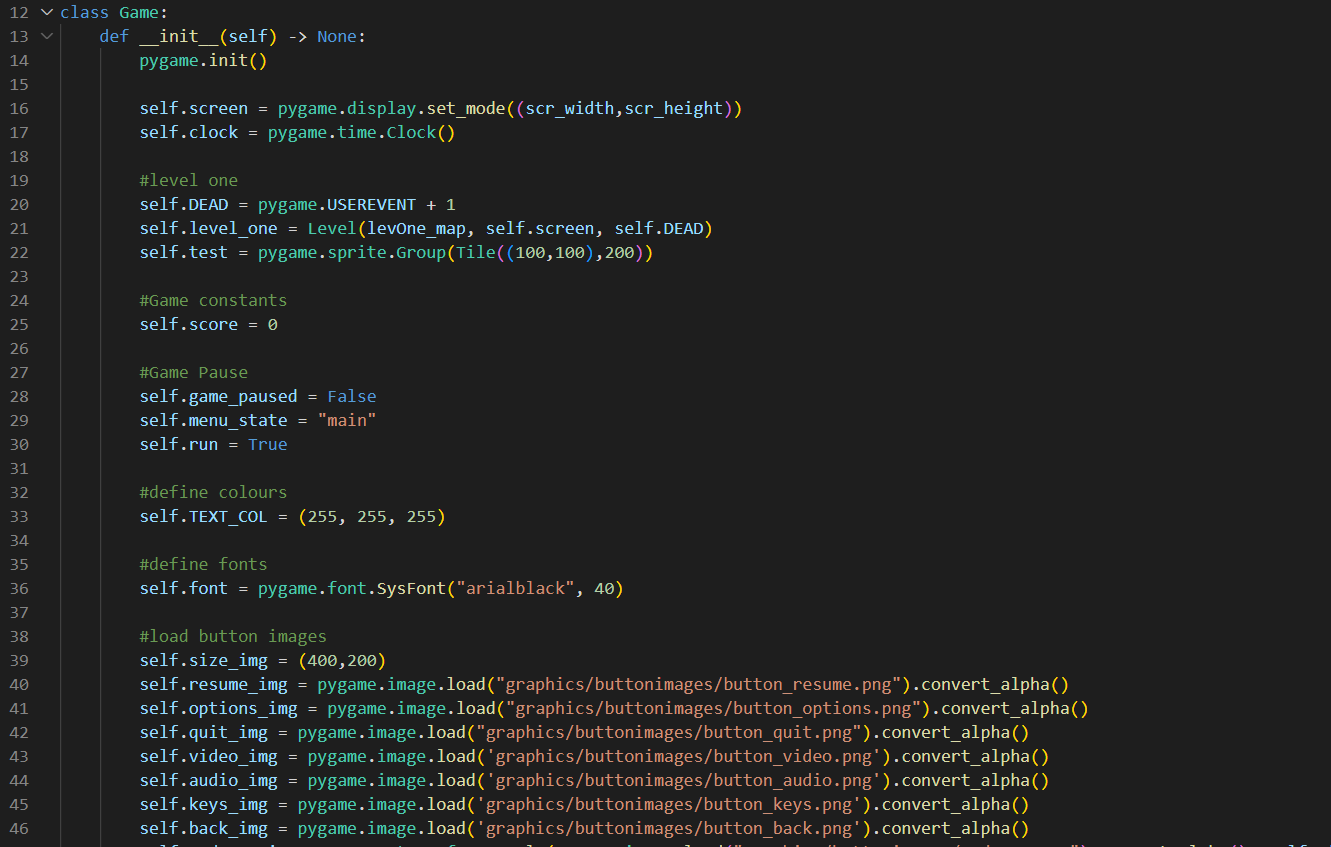
\includegraphics[width = 18cm]{game class/main1.PNG}
    \centering
\end{center}
\end{figure}\\

This is my main loop to keep the program running, however whenever you have a while loop you must have a condition or in this case an event, which will stop the loop. Here I used an event in pygame, which calls the quit function which ends the pygame loop, furthermore I also added a 'sys.exit()' to end the actual python file, which was run initially.

In the lines 20-22, I created a pygames custom event to notify the game of players death. This will be used to make the process of detecting the death of the player much simpler and convenient. On line 33, $self.TEXT-Col$ uses RGB definition of a colour, in this case having all of the colours at maximum level of 255 leads to a white colour. Similarly, $self.font$ is used to initialise a pygame font. Moreover, the lines 40-47 are used to import all the pictures that I will use to represent different menu buttons; The specific usage of the $convert-alpha()$ function is to handle images that have a transparent background and allow them to be processed by pygame.\\
\begin{figure}[H]
    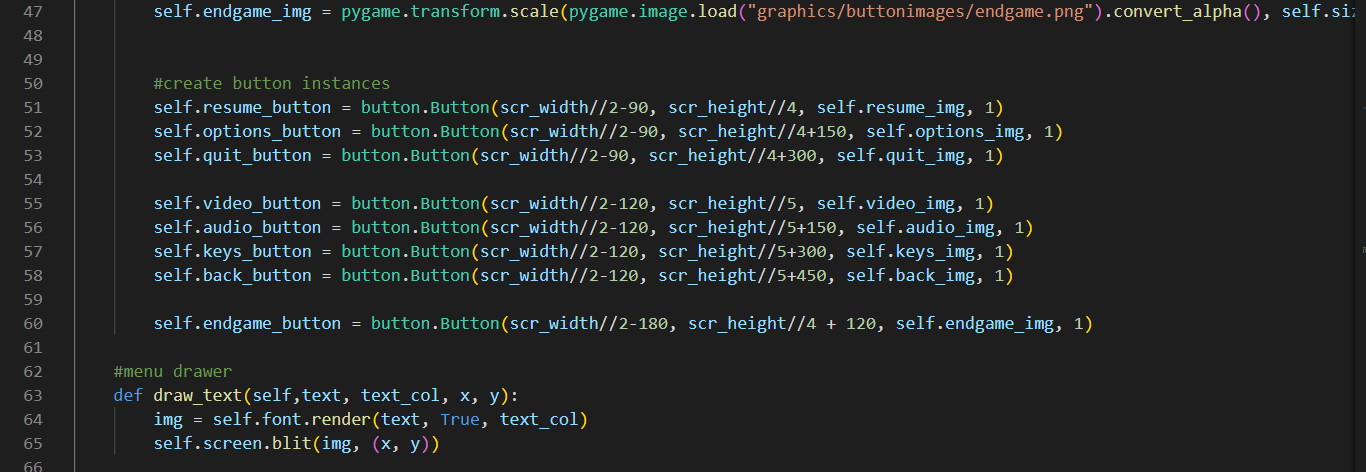
\includegraphics[width = 18cm]{game class/main2.PNG}
    \centering
\end{figure}
\vspace{3em}\\
In the lines 51-60 I created class attributes that use the pygames $button$ function to define the buttons that I will be using for the menu of the game. The parameters in pygames $button$ function define the following: divide the screen width and -90 is the x-coordinate of the button; screen height divided by 4 is the y-coordinate; self.resume-img or other image is then placed on top of the button. \\
The function $draw-text$ defined on lines 63-65 is used to draw each text on the pygames screen. The function takes in the text to be drawn, the text colour, and the x-y coordinates of placement. it then defines a local variable to hold the rendered version of the text into pygame, then it uses the pygame function $blit$ on $self.screen$ to project the rendered image on the pygame display.


The lines below:\\
\begin{figure}[H]
    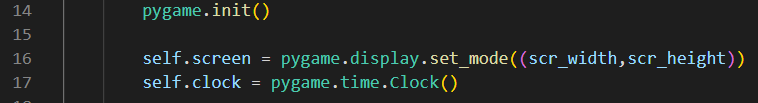
\includegraphics[width = 12cm]{game class/intitialisePyGame.PNG}
    \centering
\end{figure}
\vspace{3em}

Here I initialise the pygame, which is required to start pygame, use its classes and run the game. Next, I initialised the variable 'self.screen' to have an object that defines attributes and methods of the screen that the game will be displayed on. Finally, the variable 'self.clock', to set the clock-speed of the game, and later on, this variable will be altered or set at a constant rate.

The following code:\\
\begin{figure}[H]
    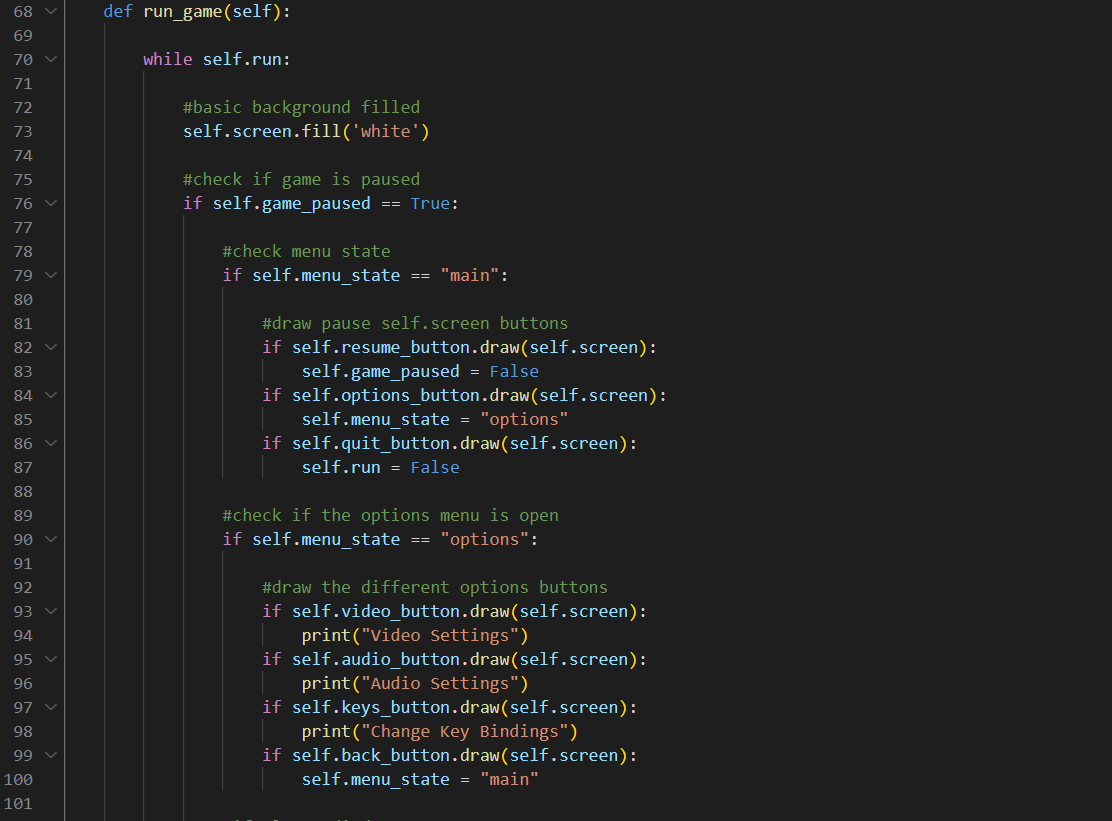
\includegraphics[width = 18cm]{game class/run1.PNG}
    \centering
\end{figure}
\begin{figure}[H]
    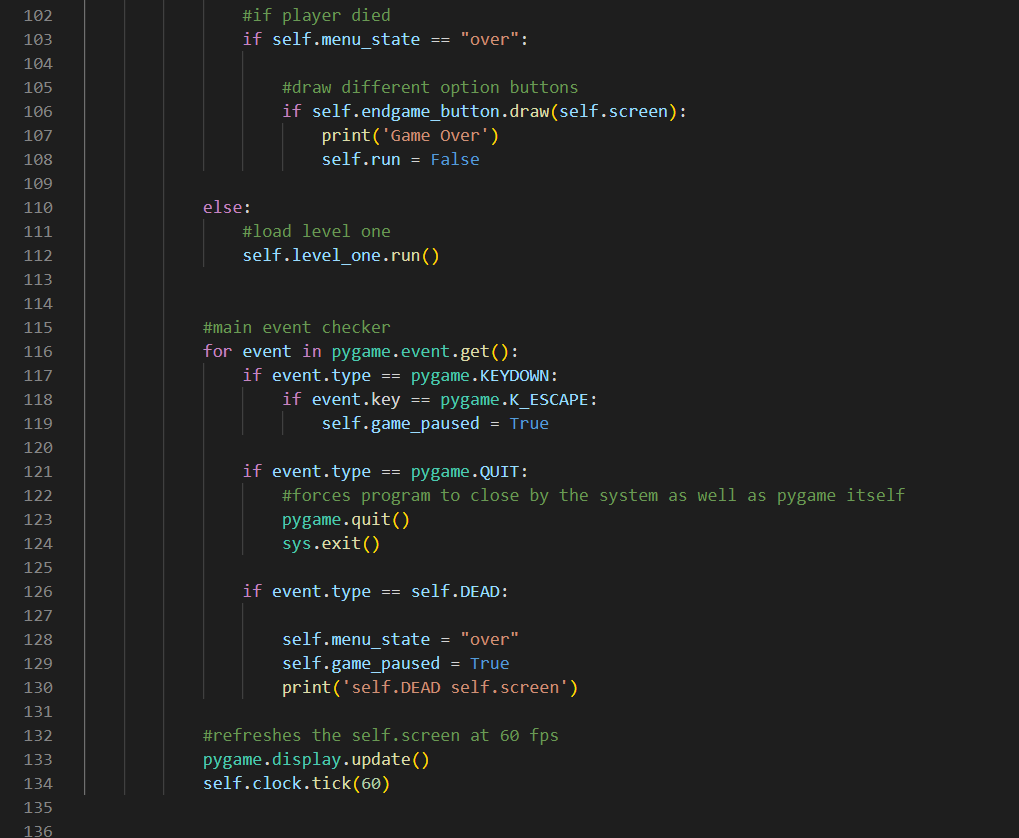
\includegraphics[width = 18cm]{game class/run2.PNG}
    \centering
\end{figure}

\vspace{3em}
Here I defined a function to keep the pygame loop running while $self.run$, Game classes attribute, is $True$.\\
In the lines 116-134, I check for updates in pygame events each loop. If event is $pygame.KEYDOWN$ and its $pygame.K-ESCAPE$, meaning the escape button is pressed, then game class attribute $self.game-paused$ will be equal to $True$. Next, if $pygame.QUIT$ then I call the $pygame.quit()$ to end the pygame loop and close the game and also call the $sys.exit()$ function to make sure the running code is closed as well. Lastly, if the event is $self.DEAD$, which is my custom pygame event, in case of the player dying, then $self.menu-state$ will be equated to 'over' and $self.game-paused$ will be equated to $True$. The use of these variables will be discussed in the following paragraph. \\

Firstly, when $self.game-paused$ is $True$ that puts the game out of the running state into one of many optional states. Next, $self.menu-state$ is a class variable that determines in which additional state the game will move onto. 
The first of those states is 'menu', representing the main menu. It consists of Resume, Options and Quit buttons. If Resume button is clicked, the main menu is closed, $self.game-paused$ is set to 'False' and the main menu is closed. If Options button is clicked, the $self.menu-state$ is set to 'options' and new set of menu is opened. Lastly, if Quit button is clicked, then $self.run$ is set to 'False' and the game is closed. The footage of the current menu is shown below:\\
\begin{figure}[H]
    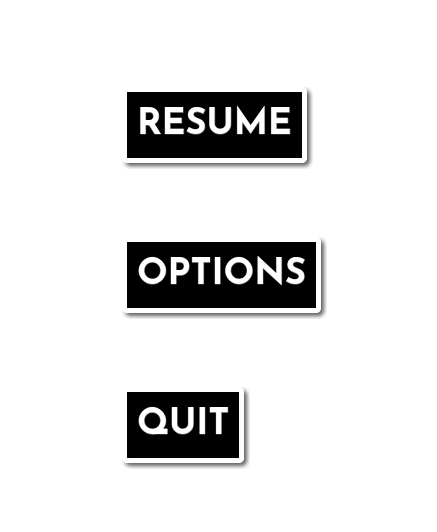
\includegraphics[width = 10cm]{game class/mainmenu.png}
    \centering
\end{figure}\\
Moreover, the further menu from clicking the Options button is also displayed below:\\
\begin{figure}[H]
    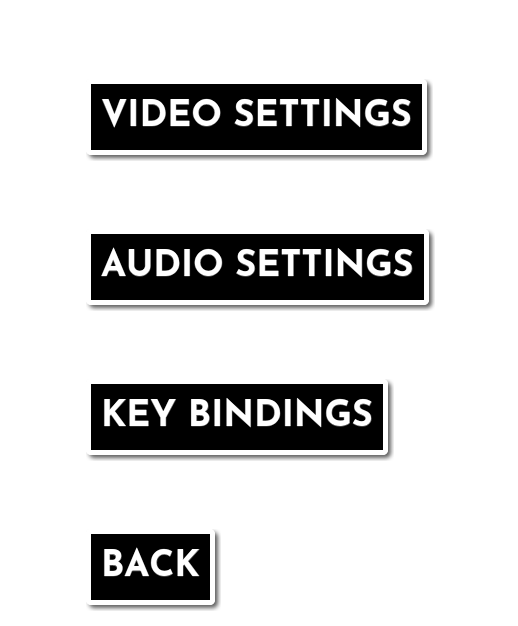
\includegraphics[width = 10cm]{game class/optmenu.png}
    \centering
\end{figure}\\
Lastly, in the lines below I define the variable x, which instantiates the class Game, and then in the following line I called the $run-game()$ function of the Game class to start the game.
\begin{figure}[H]
    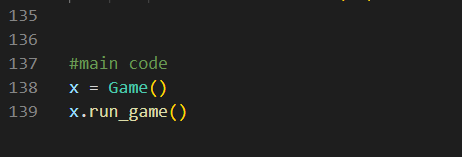
\includegraphics[width = 12cm]{game class/run3.PNG}
    \centering
\end{figure}

\subsubsection{Class Player}
I created a class for Player in a separate python file, to modularise and make the process of debugging easier. The code below demonstrates the initialisation function of the Player class.
\begin{figure}[H]
    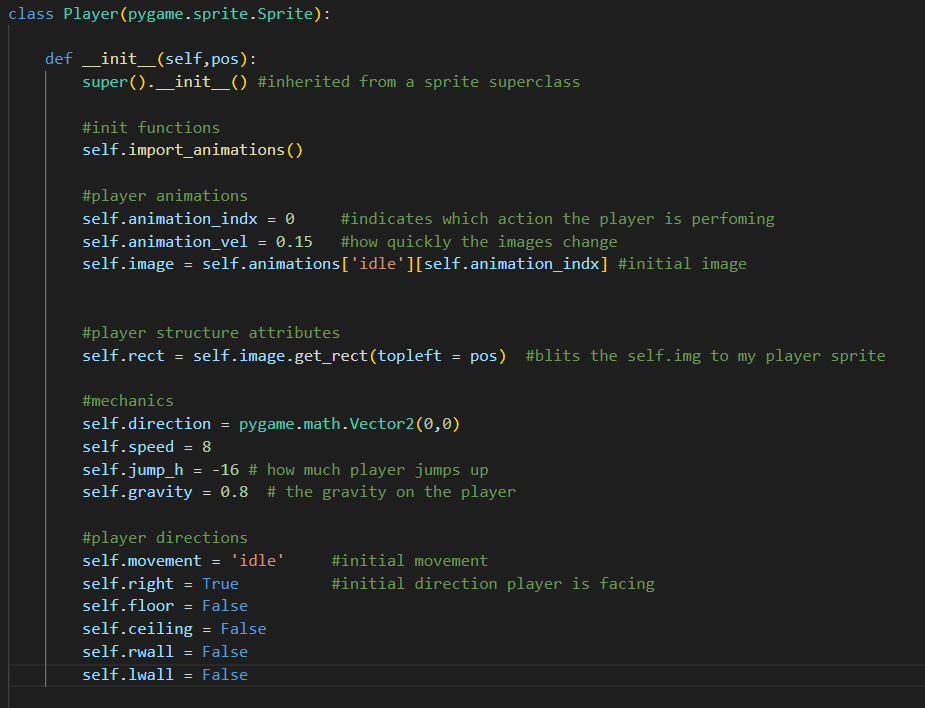
\includegraphics[width = 15cm]{player class/POne.PNG}
    \centering
\end{figure}\\
To create a pygame object, I had to call the sprite super class
The $self.import_animations()$ are calling a function within the class, which I will discuss later.  \\

The lines below:\\
\begin{figure}[H]
    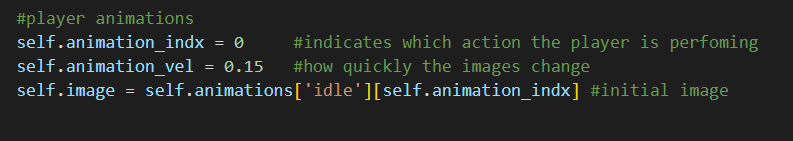
\includegraphics[width = 15cm]{player class/initPlayer1.PNG}
    \centering
\end{figure}\\
As indicated by my comments, the $self.animation-indx$ represents the current state of the player, like running or idle, which will be used to animate that player. Next, $self.animation-vel$ is the speed at which the animation or speed of changing the image on the player, I set it at 0.15, as it is an appropriate value which mitigates lag and produces the optimal performance for the game. Lastly, $self.image$ is the image which is projected onto the player object. Hence, initially it is set at status: 'idle', as all players start at idle, which makes the most logical sense. 
\newpage
\subsubsection{Parameters file}
For running the game, I created a separate python file, to store certain key elements, that are defining to the game. Having them on the separate file allows me to easily find and edit those characteristics and also increase their security, by abstracting the data in the $parameter$ file, as player cannot edit the original source used in the game.\\
\begin{figure}[H]
    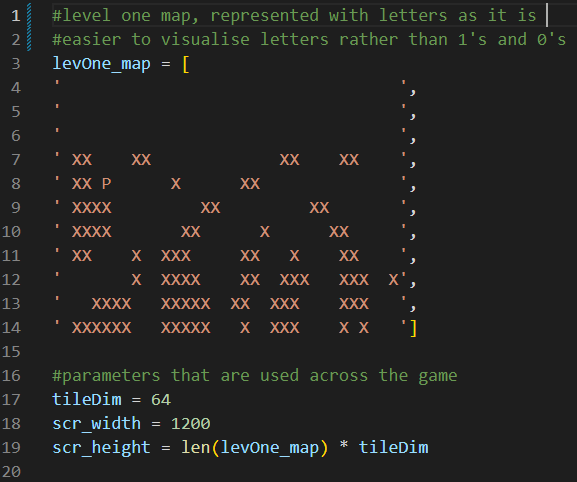
\includegraphics[width = 15cm]{Parameters/para1.png}
    \centering
\end{figure}\\
In the $levOne-map$ array, I defined the map. I used 'blank' to represent space, 'X' to represent the ground and 'P' to represent the player. I chose to use letters instead of 2's, 1's and 0's to make it easier to visually see the items in the map as it is easier for a human brain to visualise map in clear letters rather than in small numbers.\\
My game is built on abstract data type that I defined as a 'tile', which is what the game consists of, while making it easier to plan and develop the game; The variable $tileDim$ defines the dimensions of each tile. Moreover, $scr-width$ defines the width of the screen that is the window that opens on the users device, which has a constant horizontal dimensions. Lastly, $scr-height$ is defined using the size of the $levOne-map$ times by the dimension of each tile, which means this variable automatically gets corrected as you change the map, which also decreases the chances for human error and optimises the code.

\subsubsection{Level class}
To allow easier creation of other future levels and to have easier maintenance of the code I created a class to define the Level. Firstly, I required the following the imports:\\
\begin{figure}[H]
    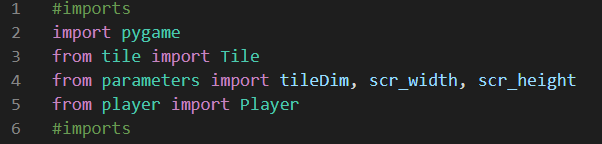
\includegraphics[width = 12cm]{Level class/loneimp.png}
    \centering
\end{figure}\\

In the following lines:\\
\begin{figure}[H]
    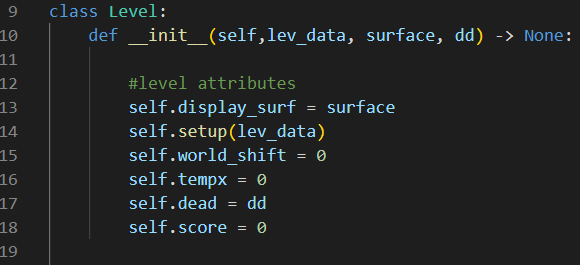
\includegraphics[width = 12cm]{Level class/loneinit.png}
    \centering
\end{figure}\\
I call the initialisation function of the Level class and set the required parameters. The $self.display-surf$ is set for surface, that will be used to define the pygame surfaces used in the game. The $self.setup(lev-data)$ calls the later defined $setup$ function of the Level class to set up and initialise the map using the supplied level data. The $self.world-shift$ is initialise set to 0, which will then be used to move the map accordingly. The rest of the variables will be used and explained in the following paragraphs.\\

In the following lines:\\
\begin{figure}[H]
    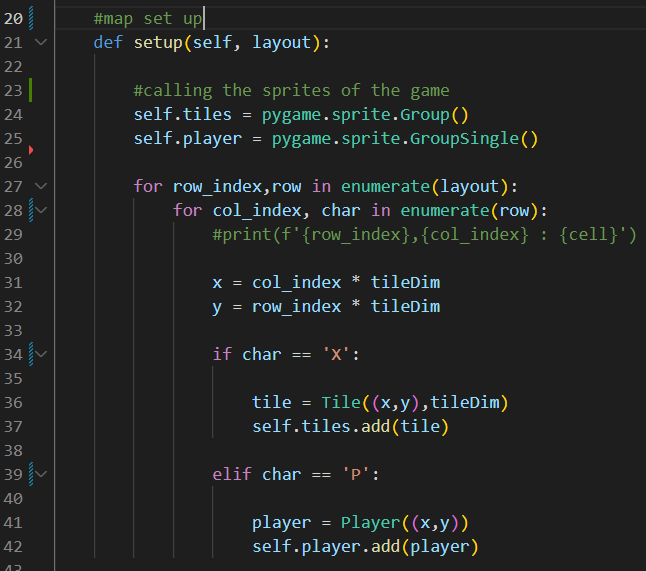
\includegraphics[width = 12cm]{Level class/lonesetup.png}
    \centering
\end{figure}\\
In the lines 23-25, I define the set up function of the level class to initialise the map of the game. The $self.tiles$, $self.player$ and $self.target$ are variables of the level class used to define the sprites representing tiles and the player of the game. Then for each character in the layout supplied, I create a tile based, with dynamic x and y coordinates depending on the characters position in the layout. However, if the character is 'X' then its a ground tile which will be added to the $self.tiles$ and if its 'P' then its a player, hence it will be added to the $self.player$.\\
\newpage
In the following lines:\\
\begin{figure}[H]
    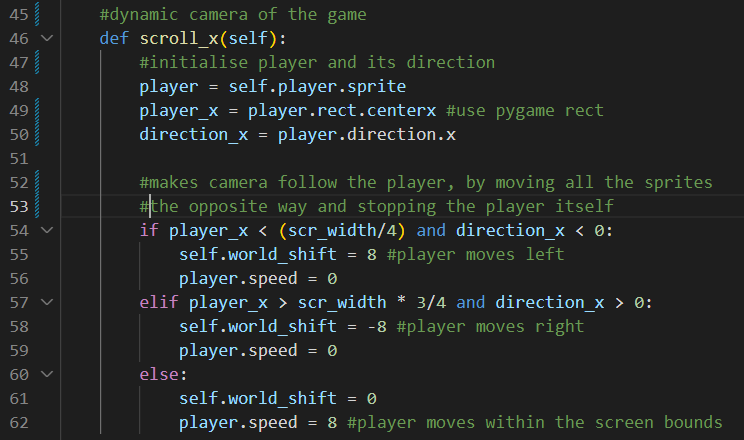
\includegraphics[width = 14cm]{Level class/scroll.png}
    \centering
\end{figure}\\
I defined a function that creates an illusion of the player moving across the map horizontally. Firstly, I need to capture data about player sprite in $player$ variable, capture x-coordinate of the player in $player-x$ and the direction of the player in $direction-x$.
Next, in the lines 54-62, I implemented the following: check if player reaches close to left or right side of the screen; If the left or right side is reached then set $player.speed = 0$, making player stop, then change the $self.world-shift =8$ or $-8$ depending on the direction of the player; Effectively, move the rest of the tiles and sprites while player is still, this visually represents the player progressing across the map horizontally. Lastly, if the player is not close to the horizontal boundaries then set $self.world-shift = 0$ and set $player.speed = 8$, hence player itself is moving across the map but the rest of the sprites are static.\\

\newpage
In the following lines:\\
\begin{figure}[H]
    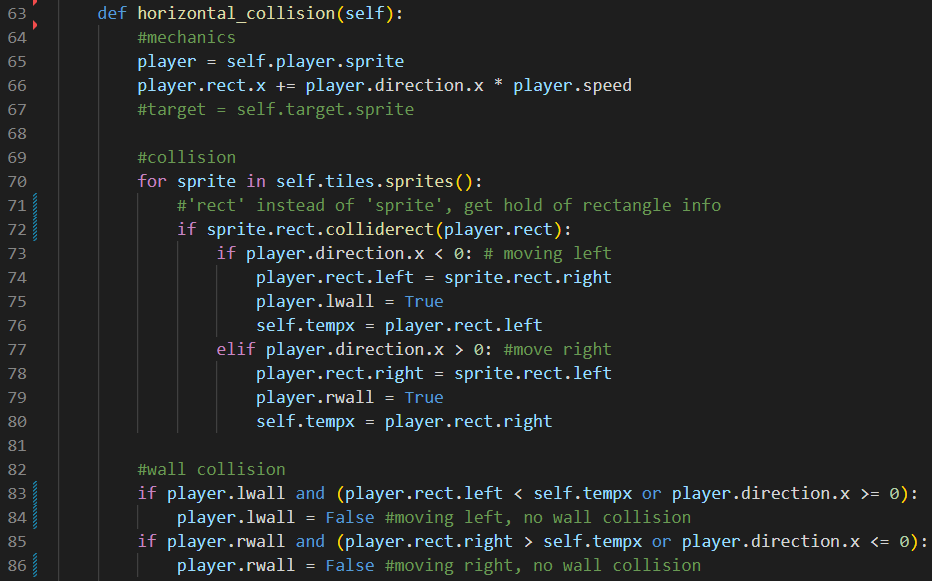
\includegraphics[width = 15cm]{Level class/horcoll.png}
    \centering
\end{figure}\\
I captured data about player sprite in $player$ variable and added the $player.direction.x * player.speed$ onto $player.rect.x$ in order to change the x location of the rectangle of the player character. Next, in the lines 70-80, I check for each sprite in the in $self.tiles$ sprite group and if their rectangular form has collided with $player.rect$ i.e. the rectangular form of the player. If the player is moving left and collides, $player.lwall$ is set to $True$, identifying collision occurred on the left side. However, if the player is moving right and collides, $player.rwall$ is set to $True$, identifying collision occurred on the right side. In each of the instances the $player.rect.left/right$ is set to equal $sprite.rect.right/left$ in order to capture the rectangle info from the collision. Lastly, in case of there being no collision I have reset the $player.lwall$ or $player.rwall$ to $False$. Now the horizontal collision takes into account all possibilities of the players horizontal actions.\\
\newpage
In the following lines:\\
\begin{figure}[H]
    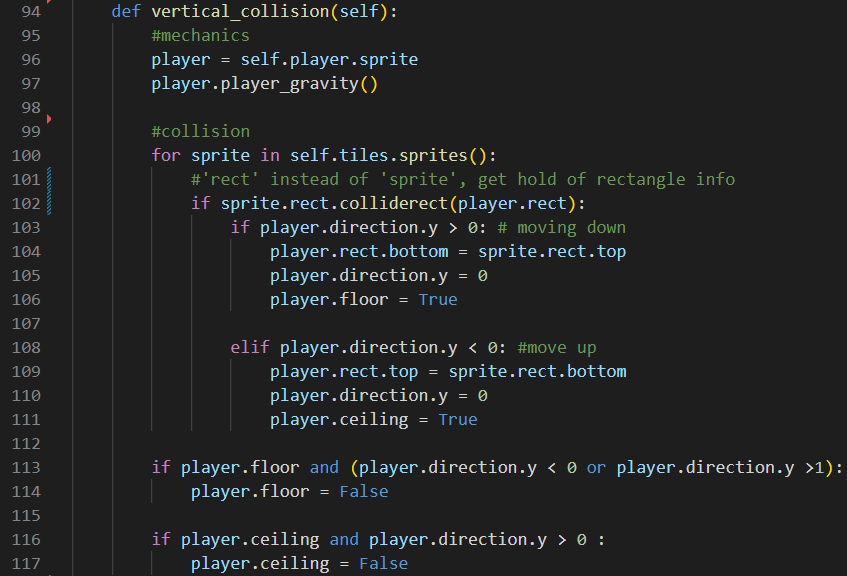
\includegraphics[width = 16cm]{Level class/vercoll.png}
    \centering
\end{figure}\\
Now, I defined a function to handle vertical collisions. Similarly to $horizontal-collision()$ I captured the player data, but now I also applied $player-gravity()$ function on the player variable. Next, for each sprite, I check if sprite has collided with the player. If so, then if $player.direction.y$ is positive then player is moving down due to the format of the coordinate system of pygame. So, I then depending on the $player.direction.y$ being above or below 0, either $player.floor$ or $player.ceiling$ is equated  to $True$. However, if there are no vertical collisions then those attributes are set to $False$. 
\subsubsection{Requirements being developed}
\subsubsection{Errors}
\subsubsection{Conclusion}

\subsection{Iteration 2}

\subsubsection{Requirements being developed}
\subsubsection{Errors}
\subsubsection{Conclusion}

\subsection{Iteration 3}
\subsubsection{Requirements being developed}
\subsubsection{Errors}
\subsubsection{Conclusion}

\section{Testing}

\section{Evaluation}

\end{document}